%Notes by Harsh Mistry 
%CS 349
%Based on Template From  https://www.cs.cmu.edu/~ggordon/10725-F12/template.tex

\documentclass[twoside]{article}
\setlength{\oddsidemargin}{0.25 in}
\setlength{\evensidemargin}{-0.25 in}
\setlength{\topmargin}{-0.6 in}
\setlength{\textwidth}{6.5 in}
\setlength{\textheight}{8.5 in}
\setlength{\headsep}{0.75 in}
\setlength{\parindent}{0 in}
\setlength{\parskip}{0.1 in}
\usepackage{amsmath,amsfonts,graphicx}
\newcounter{lecnum}
\renewcommand{\thepage}{\thelecnum-\arabic{page}}
\renewcommand{\thesection}{\thelecnum.\arabic{section}}
\renewcommand{\theequation}{\thelecnum.\arabic{equation}}
\renewcommand{\thefigure}{\thelecnum.\arabic{figure}}
\renewcommand{\thetable}{\thelecnum.\arabic{table}}
\newcommand{\lecture}[4]{
   \pagestyle{myheadings}
   \thispagestyle{plain}
   \newpage
   \setcounter{lecnum}{#1}
   \setcounter{page}{1}
   
   
%Info Box 
   \begin{center}
   \framebox{
      \vbox{\vspace{2mm}
    \hbox to 6.28in { {\bf CS 349 - User Interfaces
	\hfill Winter 2018} }
       \vspace{4mm}
       \hbox to 6.28in { {\Large \hfill Lecture #1: #2  \hfill} }
       \vspace{2mm}
       \hbox to 6.28in { {\it Lecturer: #3 \hfill Notes By: #4} }
      \vspace{2mm}}
   }
   \end{center}
   
   \markboth{Lecture #1: #2}{Lecture #1: #2}



 
}

\renewcommand{\cite}[1]{[#1]}
\def\beginrefs{\begin{list}%
        {[\arabic{equation}]}{\usecounter{equation}
         \setlength{\leftmargin}{2.0truecm}\setlength{\labelsep}{0.4truecm}%
         \setlength{\labelwidth}{1.6truecm}}}
\def\endrefs{\end{list}}
\def\bibentry#1{\item[\hbox{[#1]}]}

\newcommand{\fig}[3]{
			\vspace{#2}
			\begin{center}
			Figure \thelecnum.#1:~#3
			\end{center}
	}
	
\graphicspath{ {images/} }

\newtheorem{theorem}{Theorem}[lecnum]
\newtheorem{lemma}[theorem]{Lemma}
\newtheorem{ex}[theorem]{Example}
\newtheorem{proposition}[theorem]{Proposition}
\newtheorem{claim}[theorem]{Claim}
\newtheorem{corollary}[theorem]{Corollary}
\newtheorem{definition}[theorem]{Definition}
\newenvironment{proof}{{\bf Proof:}}{\hfill\rule{2mm}{2mm}}
\newcommand\E{\mathbb{E}}


%Start of Document 
\begin{document}

\lecture{5}{January 12, 2018}{Keiko Katsuragawa}{Harsh Mistry}

\section{Events}


\subsection{Event Driven Programming}
In event driven programming nothing happens unless some other event occurs first. i.e
\begin{itemize}
\item User presses a key,
\item User moves the mouse
\item Window is resized/closed/covered
\item Timer expires
\end{itemize}

\subsubsection{Events Defined}
\begin{itemize}
\item English : An observable occurrence, often extraordinary occurrence
\item User Interface Architecture : A message to notify an application that something happened
\item Examples 
\begin{itemize}
\item Keyboard 
\item Pointer Events 
\item Window crossing
\item Input focus
\item Window events
\item Timer
\end{itemize}
\end{itemize}

\subsubsection{Role of the Base Window System}
\begin{itemize}
\item Collect event information
\item Put relevant information in a known structure
\item Order teh events by time
\item Decide which application/window should get event 
\item Deliver the event
\item Some events come from teh user via the underlying hardware; some from the window manager
\end{itemize}

\subsubsection{Receiving events}
\begin{itemize}
\item In X windows, applications get the next event using : \verb|XNextEvent(Display* display, XEvent* evt)|
\begin{itemize}
\item Gets and removes teh next event in the queue 
\item \textbf{If empty, it blocks until another event arrives}
\end{itemize}
\item To avoid blocking you can use \verb|XPending(Display* display)|
\end{itemize}

\subsubsection{Selecting input events to listen to}
\begin{center}
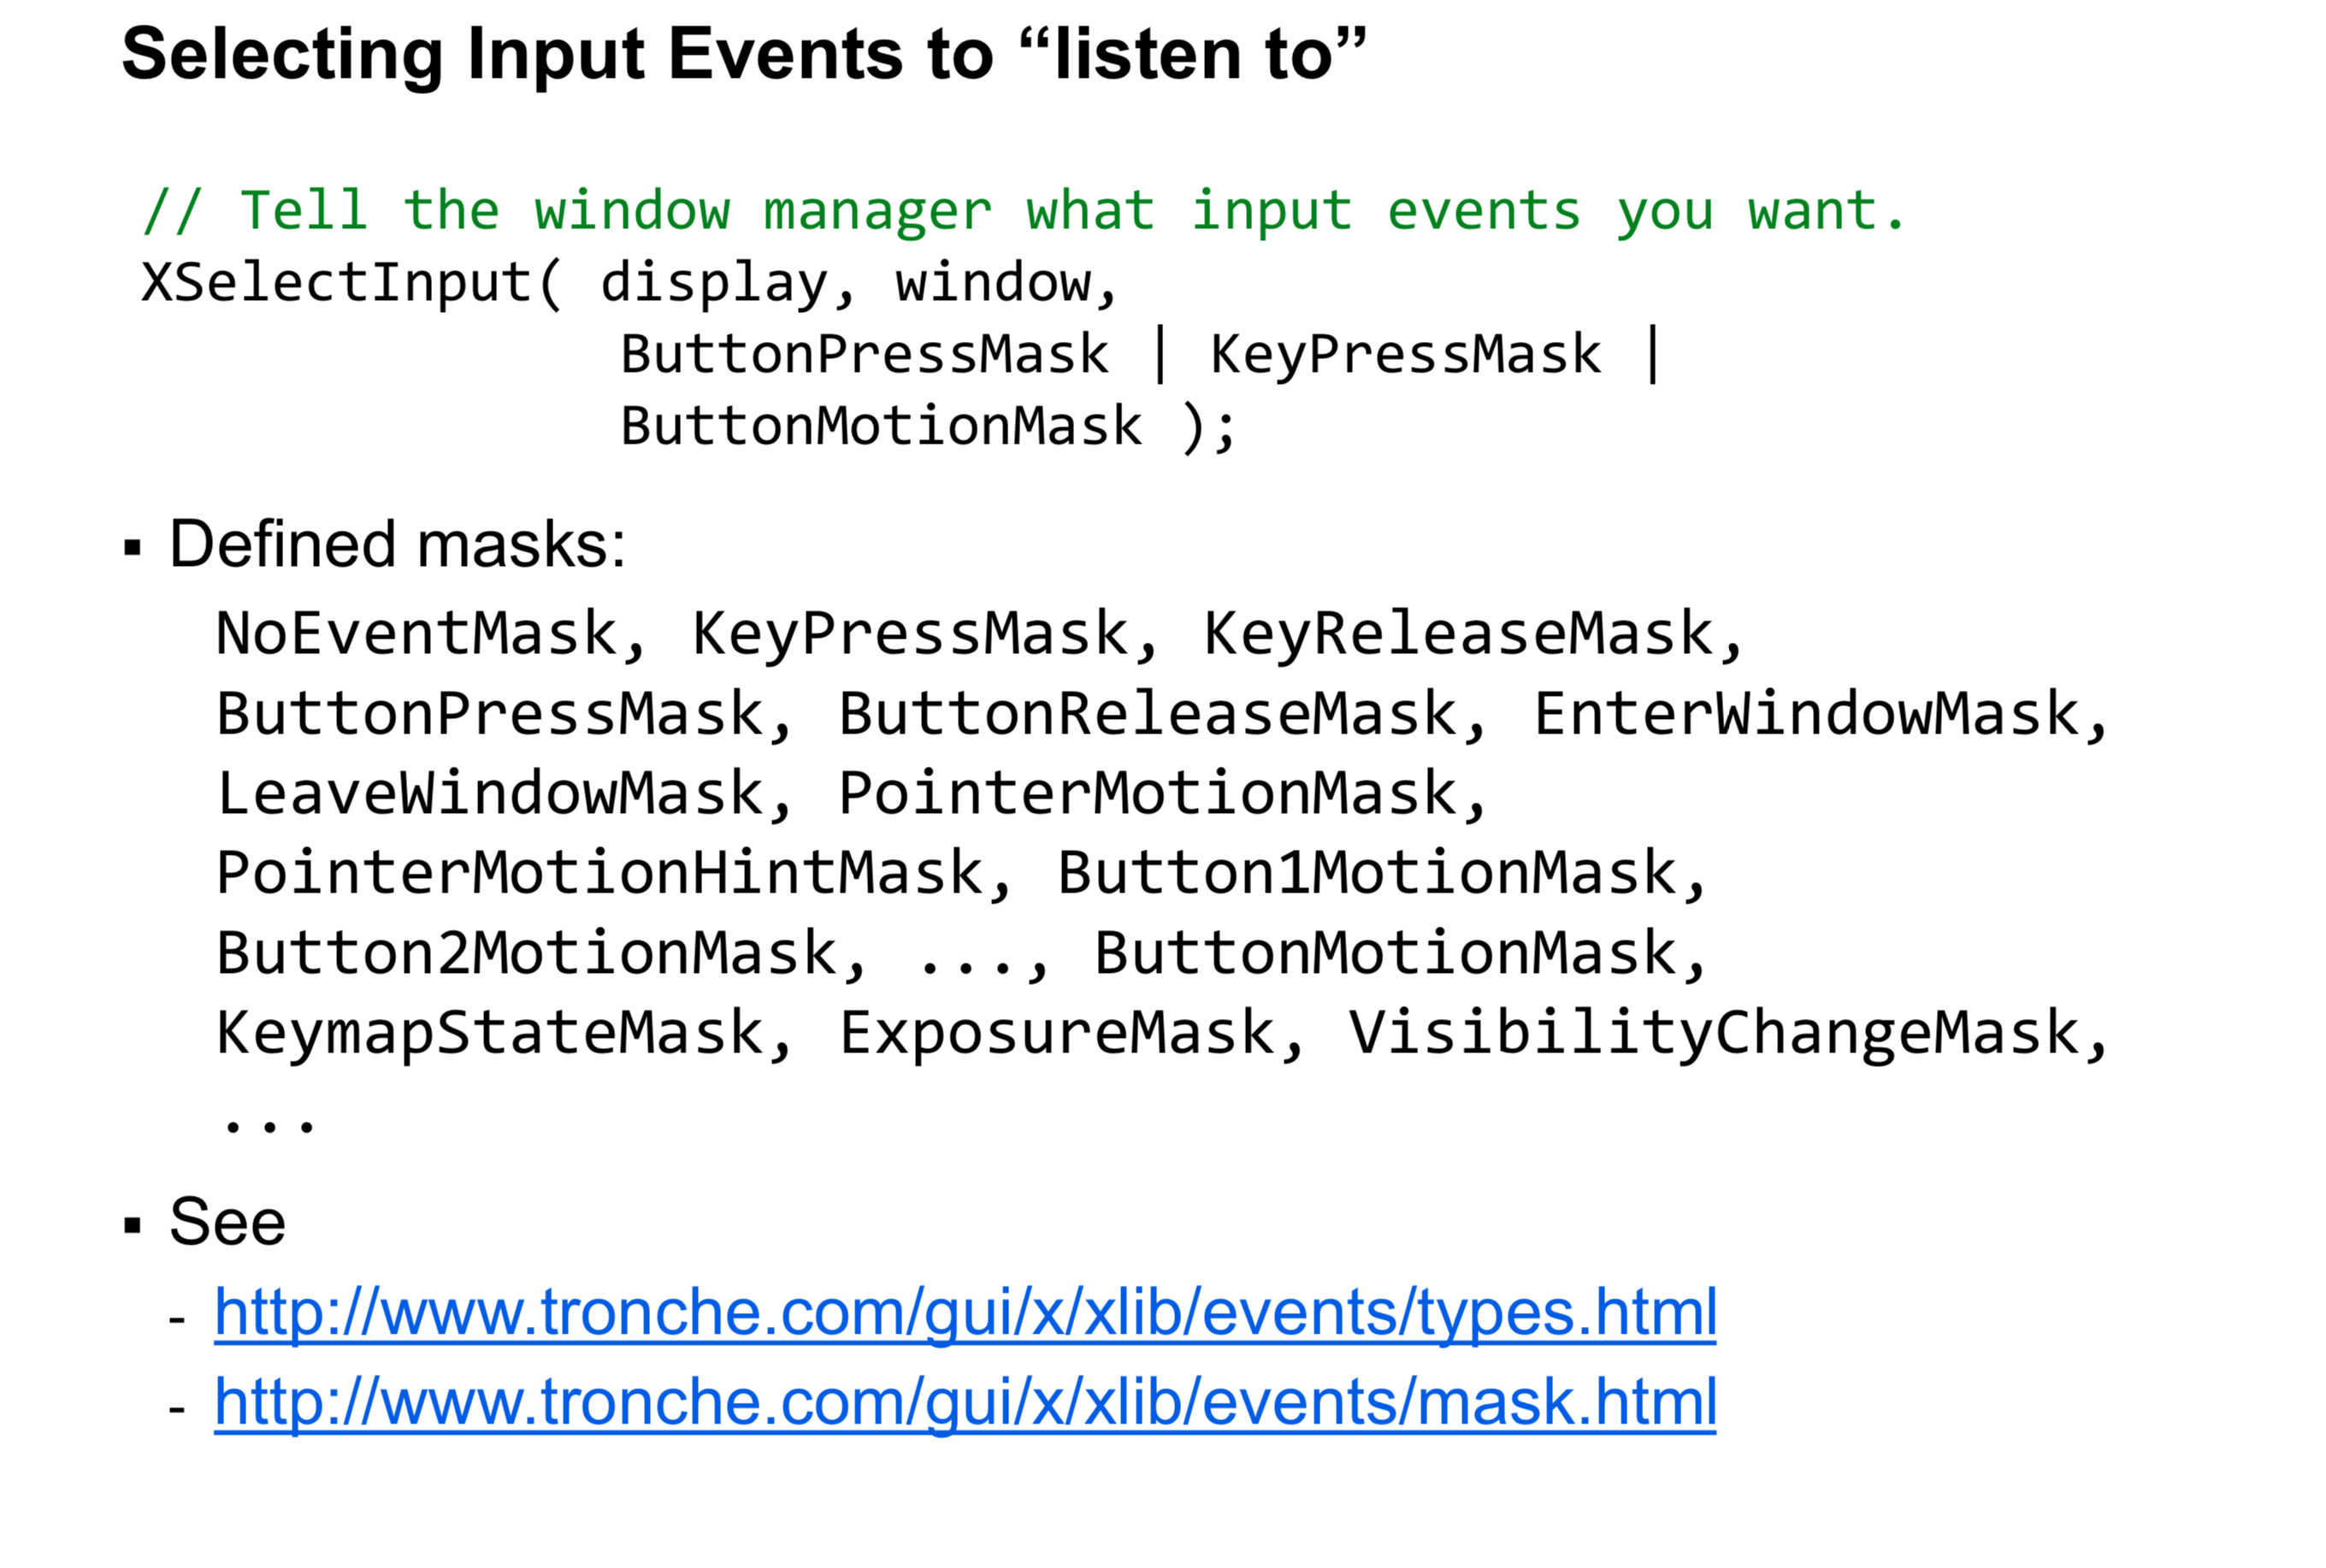
\includegraphics[scale=0.3]{6}\\
Slide Taken From Lecture
\end{center}
\newpage 
\subsubsection{Event Structure}
\begin{center}
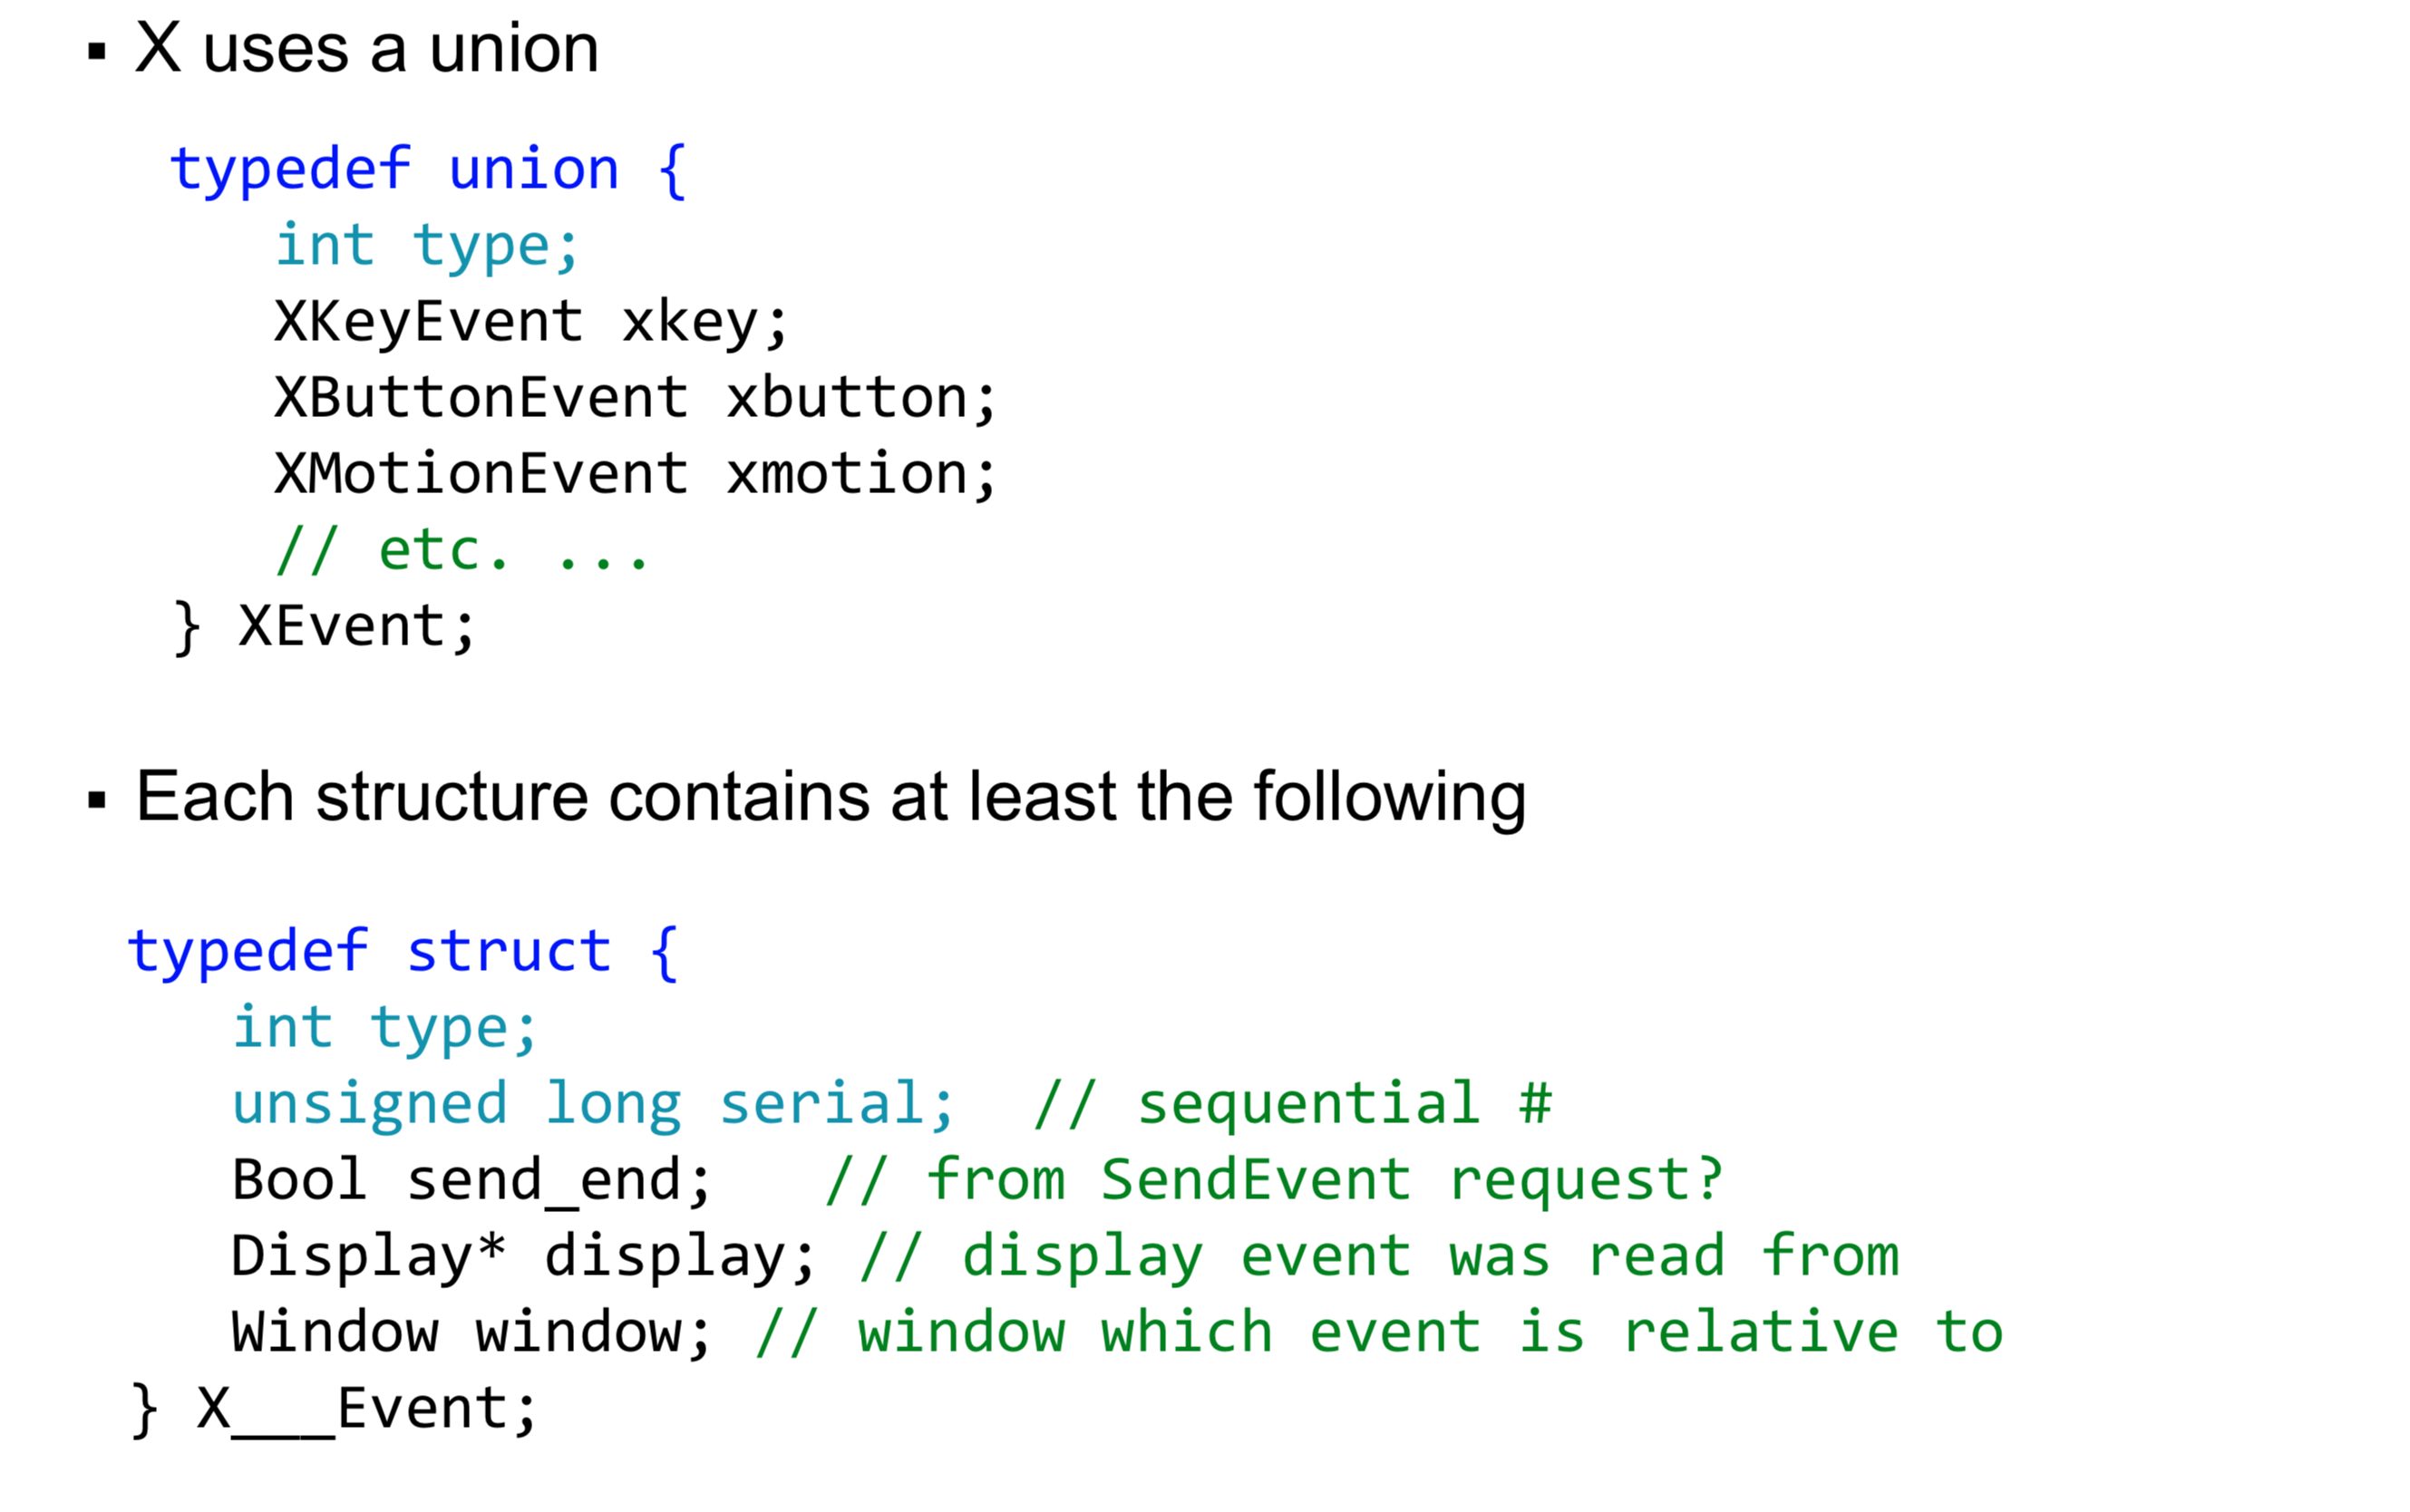
\includegraphics[scale=0.3]{7}\\
Slide Taken From Lecture
\end{center}

\subsection{Animation}
Animation is the simulation of movement created by displaying a series of pictures, or frames

\begin{center}
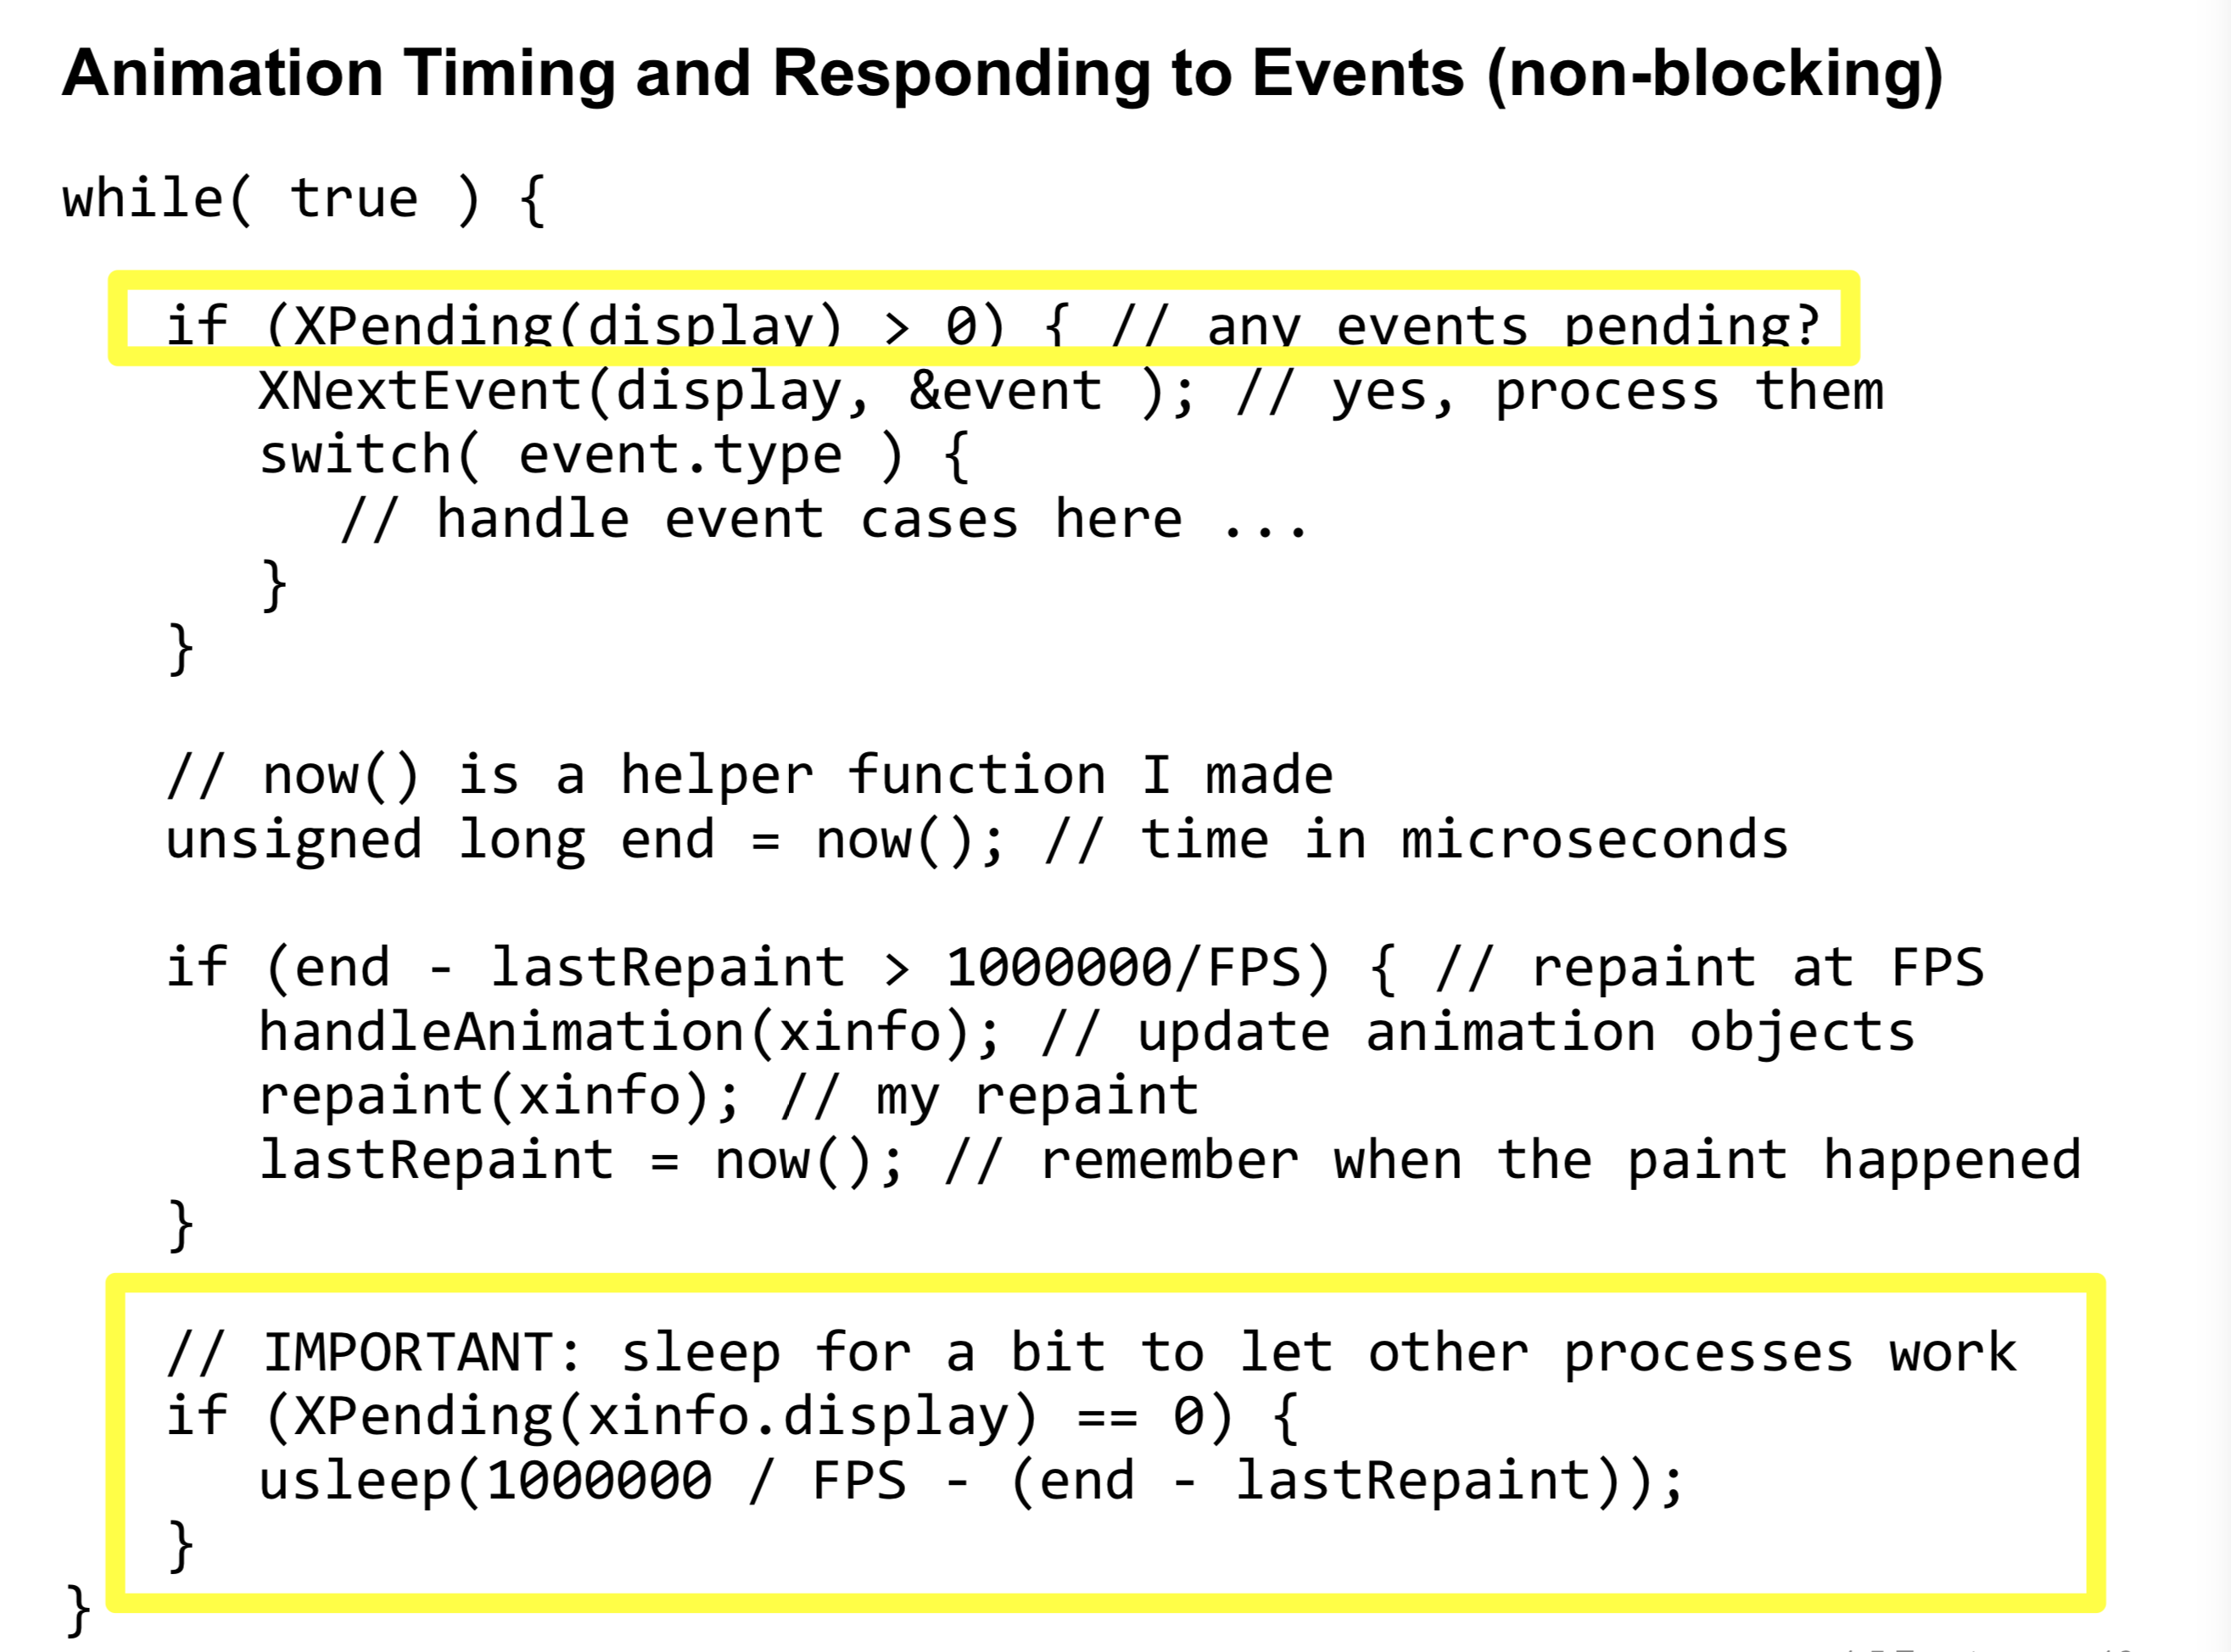
\includegraphics[scale=0.2]{8}\\
Slide Taken From Lecture
\end{center}

\subsection{Double Buffering}
Flickering can occur when an intermediate image is on the display. To resolve this we can use double buffering, which involves rendering images off screen to a buffer and then fast copying the buffer to the screen 

\begin{center}
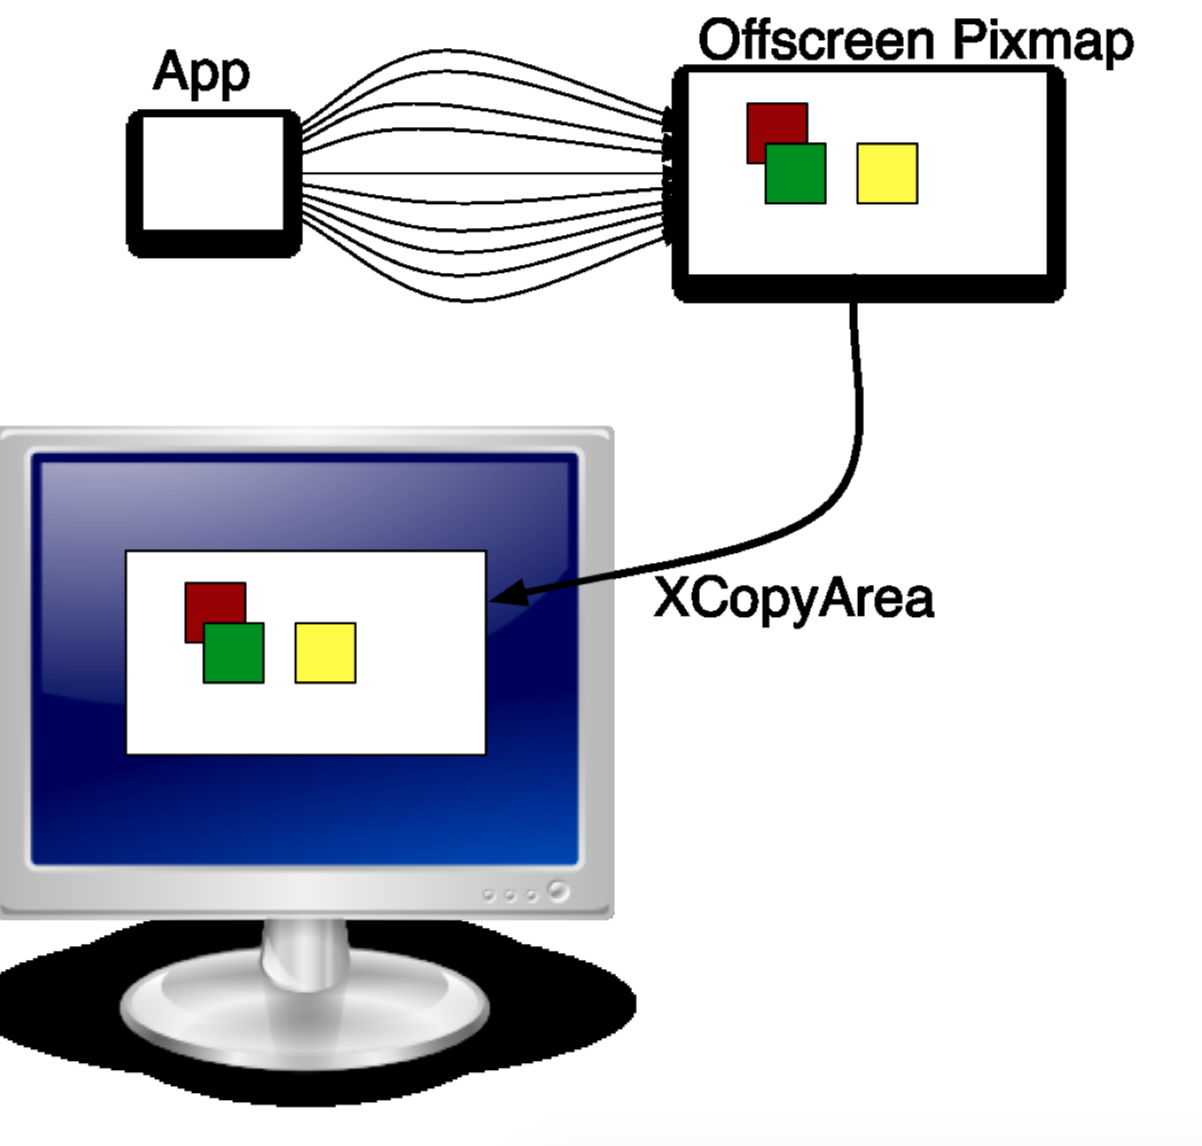
\includegraphics[scale=0.2]{9}\\
Graphic Taken From Lecture
\end{center}

\subsection{Painting Advice}
\begin{itemize}
\item Keep it simple
\begin{itemize}
\item Clear everything and redraw each frame
\item Use advanced methods, only if you really need them for performance
\end{itemize}
\item Don't repaint too often. Consider adding a "someChanged" bool flag
\item Don't flush too often
\end{itemize}


\end{document}





